\section{Evaluation}\seclabel{Evaluation}
In this section, we describe and evaluate Lucy: a prototype implementation of
our decision procedures and system models.
% We evaluate Lucy by answering the following questions:
% \begin{itemize}
%   \item
%     How practical is the interactive invariant-confluence decision procedure?
%     Can we use it to classify real-world transactions and invariants?
%   \item
%     How practical is segmented invariant-confluence? Are real-world workloads
%     amenable to segmentation?
%   \item
%     How efficient is the interactive invariant-confluence decision procedure?
%   \item
%     How efficiently can we replicate a segmented invariant-confluent object as
%     compared to alternative approaches like replicating with weak or strong
%     consistency?
%   \item
%     How does the performance of replicating a segmented invariant-confluence
%     object vary as we vary the workload, segmentation, and replication factor?
% \end{itemize}

\subsection{Implementation}
Lucy includes an implementation of the interactive decision procedure described
in \algoref{InteractiveDecisionProcedure}, an implementation of a decision
procedure which checks criteria (1) - (4) from \thmref{LatticeProperty}, and an
implementation of the decision procedure described in
\algoref{ArbitraryStartInteractiveDecisionProcedure}. The decision procedures
are implemented in roughly 2,500 lines of Python. Users specify objects,
transactions, and invariants in a small Python DSL and interact with the
interactive decision procedures using an interactive Python console. We use
Z3~\cite{de2008z3} to implement our invariant-closure decision procedure,
compiling an object and invariant into a formula that is satisfiable if and
only if the object is \emph{not} invariant-closed. If the object is
invariant-closed, then Z3 concludes that the formula is unsatisfiable.
Otherwise, if the object is not invariant-closed, then Z3 produces a
counterexample witnessing the satisfiability of the formula.

Lucy also includes an implementation of the invariant-confluence and
segmented-invariant confluence system models in roughly 3,500 lines of C++.
Users specify objects, transactions, invariants, and segmentations in C++. Lucy
then replicates the objects using segmented invariant-confluence (or
invariant-confluence if the segmentation contains a single segment without any
disallowed transactions). Clients send every transaction request to a randomly
selected server. When a server receives a transaction request, it executes
\algoref{TxnExecution} to attempt to execute the transaction locally. If the
transaction requires global coordination, then the server forwards the
transaction request to a predetermined leader. When the leader receives a
transaction request, it sends a coordination request to all other servers. When
a server receives a coordination request from the leader, it stops processing
transactions and sends the leader its state in a coordination reply. When the
leader receives coordination replies from all other servers, it executes the
transaction, and then sends its state to the other servers. When a server
receives a new state, it adopts the state, computes its new active segment, and
resumes normal processing. After every 100 transactions processed, a server
sends a merge request to a randomly selected server. Merge requests are tagged
with a monotonically increasing epoch number that is incremented by the master
after every round of global coordination. This allows servers to discard merge
requests from previous epochs.

Lucy can also replicate an object with eventual consistency and with
linearizability. With eventual consistency, clients send every transaction
request to a randomly selected server. The server executes the transaction
locally and returns immediately to the client, sending merge requests after
every 100 transactions. With linearizability, clients send every transaction
request to a predetermined leader. The leader relays the transaction request to
all other servers, and when it receives replies from them, it executes the
transaction and replies to the client. This communication pattern mimics the
``normal operation'' of state machine replication protocols like
Paxos~\cite{lamport1998part} and Viewstamped
Replicated~\cite{liskov2012viewstamped}. In
\secref{SegmentedInvariantConfluenceEval}, we compare the performance of
replicating with segmented invariant-confluence against the performance of
replicating with eventual consistency and linearizability.

Because fault-tolerance is largely an orthogonal concern to
invariant-confluence, Lucy is implemented without fault-tolerance. It would be
straightforward to add fault-tolerance to Lucy, but it would not affect our
discussions or evaluation, so we leave it for future work. Moreover, users
currently have to specify their workloads in Python (for the decision
procedures) and C++ (for the runtime). In the future, we plan on removing this
redundancy.

\subsection{Decision Procedures}
We now evaluate the practicality and efficiency of our decision procedure
prototypes. We begin by demonstrating the decision procedure on a handful of
simple, yet practical examples. We then, discuss TODO

% \todo{Bank account with and without decrements.}
% \todo{Auction example.}
% \todo{Foreign keys with and without deletions.}
% \subsection{TPC and Feral}
% \todo{See which of the Feral and TPC transactions we can determine automatically}
\example[$\ints^2$]\examplelabel{TwoIntsEval}
We begin with a minimal working example. Consider again our recurring example
of $\ints^2$ from \exampleref{Z2}. The Python code used to describe the object,
transactions, and invariant is given in \figref{Z2Code}. When we call
\python{checker.check()}, the interactive decision procedure produces
a counterexample in less than a tenth of a second.  After we label the
counterexample and refine the invariant with $y \leq 0$, the interactive
decision procedure determines that the object is invariant-confluent, again, in
less than a tenth of a second. Note that the object is invariant-confluent but
\emph{not} invariant-closed, so prior work that relies on invariant-closure
alone to determine invariant-confluence would not be able to identify this
example as invariant-confluent.

\begin{figure}[ht]
  \begin{Python}[gobble=4]
    checker = InteractiveInvariantConfluenceChecker()
    x = checker.int_max('x', 0) # An int, x, merged by max.
    y = checker.int_max('y', 0) # An int, y, merged by max.
    checker.add_transaction('increment_x', [x.assign(x + 1)])
    checker.add_transaction('decrement_y', [y.assign(y - 1)])
    checker.add_invariant(x * y <= 0)
    checker.check()
  \end{Python}
  \caption{\exampleref{TwoIntsEval} specification}\figlabel{Z2Code}
\end{figure}

\example[Foreign Keys]\examplelabel{ForeignKeysEval}
A 2P-Set $X = (A_X, R_X)$ is a set CRDT composed of a set of additions $A_X$
and a set of removals $R_X$~\cite{shapiro2011comprehensive}. We view the state
of the set $X$ as the difference $A_X - R_X$ of the addition and removal sets.
To add an element $x$ to the set, we add $x$ to $A_X$. Similarly, to remove $x$
from the set, we add it to $R_X$. The merge of two 2P-sets is a pairwise union
(i.e. $(A_X, R_X) \join (A_Y, R_Y) = (A_X \cup A_Y, R_X \cup R_Y)$).

We can use 2P-sets to model a simple relational database with foreign key
constraints. Let object $O = (X, Y) = ((A_X, R_X), (A_Y, R_Y))$ consist of a
pair of two 2P-Sets $X$ and $Y$, which we view as relations. Our invariant $X
\subseteq Y$ (i.e. $(A_X - R_X) \subseteq (A_Y - R_Y)$) models a foreign key
constraint from $X$ to $Y$. We ran our decision procedure on the object with
initial state $((\emptyset, \emptyset), (\emptyset, \emptyset))$ and
transactions that allow arbitrary insertions and deletions into $X$ and $Y$.
After less than a tenth of a second, the decision procedure produced a
reachable counterexample witnessing the fact that the object is not
invariant-confluent. A concurrent insertion into $X$ and deletion from $Y$ can
lead to a state which violates the invariant. This object is not
invariant-confluent and therefore not invariant-closed. Thus, previous tools
depending on invariant-closure as a sufficient condition would be unable to
conclude definitively that the object is \emph{not} invariant-confluent.

We also reran the decision procedure, but this time with insertions into $X$
and deletions from $Y$ disallowed. In less than a tenth of a second, the
decision procedure correctly deduced that the object is now
invariant-confluent. These results were manually proven
in~\cite{bailis2014coordination}, but our tool was able to confirm them
automatically in a negligible amount of time.

\example[Auction]\examplelabel{AuctionEval}
We now consider a simple auction system introduced in~\cite{gotsman2016cause}.
Our object consists of a set $B$ of integer-valued bids and a optional winning
bid $w$. Initially, $B = \emptyset$ and $w = \bot$ (indicating that there is no
winning bid yet) and we merge states by taking the union of $B$ and the maximum
of $w$ (where $\bot < n$ for all integers $n$). One transaction $t_b$ places a bid
$b$ by inserting it into $B$. Another transaction $t_\text{close}$ closes the
auction and sets $w$ equal to the largest bid in $B$. Our invariant is that if
the auction is closed (i.e.\ $w \neq \bot$), then $w = \max(B)$. We ran our
decision procedure on this example and in a third of a second, it produced a
reachable counterexample witnessing the fact that the object is not
invariant-confluent.  If we concurrently close the auction and place an large
bid, then we can end up in a state in which the auction is closed, but there is
a higher bid in $B$.

We then segmented our object as follows. The first segment $(\setst{(B, w)}{w =
\bot}, \setst{t_b}{b \in \ints})$ allows any bidding transaction so long as the
bid is open. The second segment $(\setst{B, w}{I \cap w \neq \bot}, \emptyset)$
includes all auctions which have already been closed and forbids all
transactions. This segmentation captures the intuition that bids should be
permitted only when the auction is open. We ran our segmented
invariant-confluence decision procedure on this example, and it was able to
deduce without any human interaction that the example was segmented
invariant-confluent in less than a tenth of a second.

\example[Escrow Transactions]\examplelabel{EscrowTransactionsEval}
Escrow transactions are a concurrency control technique that allows a database
to execute transactions that increment and decrement numeric values with more
concurrency than is otherwise possible with general-purpose techniques like
two-phase locking~\cite{o1986escrow}. The main idea is that a portion of the
numeric value is put in escrow, after which a transaction can freely decrement
the value so long as it is not decremented by more than the amount that has
been escrowed. We now show how segmented invariant-confluence can be used to
implement escrow transactions.

Consider again the PN-Counter $s = (p_1, p_2, p_3), (n_1, n_2, n_3)$ from
\exampleref{CounreachableExample} replicated on three servers with transactions
to increment and decrement the PN-Counter. In
\exampleref{CounreachableExample}, we found that concurrent decrements violate
invariant-confluence which led us to a segmentation which prohibited concurrent
decrements. We now propose a new segmentation with escrow amount $k$ that will
allow us to perform concurrent decrements that respect the escrowed value. The
first segment $(\setst{(p_1, p_2, p_3), (n_1, n_2, n_3)}{p_1, p_2, p_3 \geq k
\land n_1, n_2, n_3 \leq k}, T)$ allows for concurrent increments and
decrements so long as every $p_i \geq k$ and every $n_i \leq k$. Intuitively,
this segment represents the situation in which every server has escrowed a
value of $k$. They can decrement freely, so long as they don't exceed their
escrow budget of $k$. The second segment is the one presented in
\exampleref{CounreachableExample} which prohibits concurrent decrements. We ran
our decision procedure on this example and it concluded that it was segmented
invariant-confluent in less than a tenth of a second and without any human
interaction.

\textbf{TPC-C and Feral Concurrency Control.}

TODO

\subsection{Segmented Invariant Confluence}%
\seclabel{SegmentedInvariantConfluenceEval}
Now, we evaluate the performance of replicating an object with segmented
invariant-confluence as compared to replicating it with eventual consistency or
linearizability. We begin with two benchmarks that demonstrate the same
concept: the performance of segmented invariant-confluent replication varies
with the amount of global coordination induced by either (a) performing a
transaction that is disallowed within a segment or (b) transitioning between
segments.

\begin{figure}[ht]
  \centering

  \begin{subfigure}[c]{\columnwidth}
    \centering
    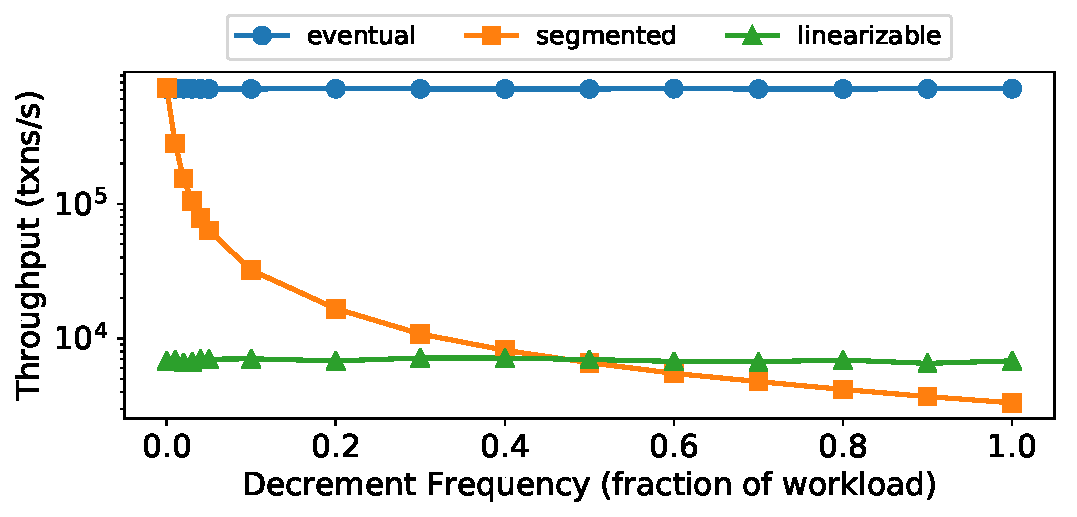
\includegraphics[width=\columnwidth]{figures/vary_withdraws.pdf}
  \end{subfigure}
  \begin{subfigure}[c]{\columnwidth}
    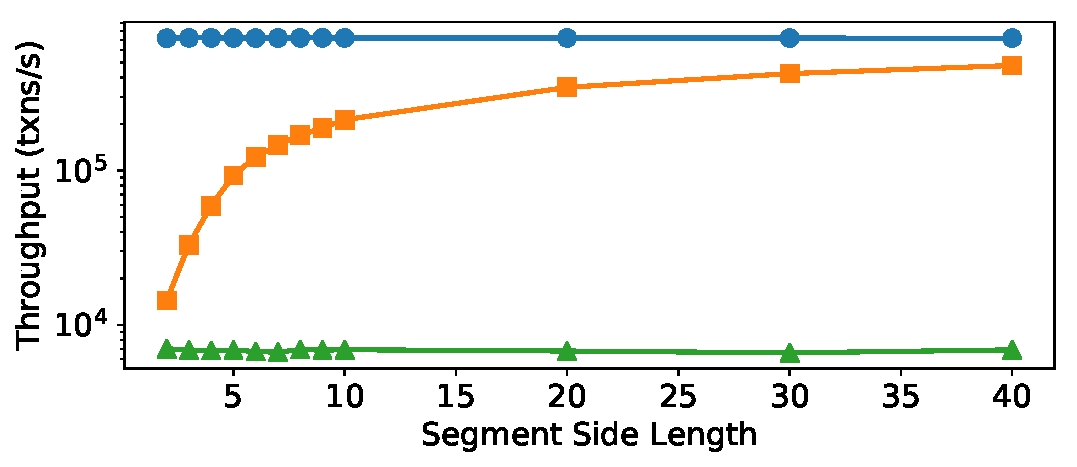
\includegraphics[width=\columnwidth]{figures/vary_segments.pdf}
  \end{subfigure}

  \caption{%
    Segmented invariant-confluent replication throughput versus coordination,
    induced by executing disallowed transactions (top) and by transitioning
    across segments (bottom).
  }\figlabel{ThroughputVsGlobalSyncs}
\end{figure}

\begin{benchmark}\benchlabel{VaryWithdraws}
Consider again the PN-Counter from \exampleref{CounreachableExample} and the
corresponding transactions, invariants, and single-segment segmentation that
forbids concurrent decrements. We replicate this object on 32 servers
deployed on 32 m5.xlarge EC2 instances within the same availability zone.  Each
server has three colocated clients that issue deposit and withdrawal
transactions. We replicate the object with eventual consistency, segmented
invariant-confluence, and linearizability and measure the system's total
throughput as we vary the fraction of client requests that are withdrawals. The
results are shown in the top of \figref{ThroughputVsGlobalSyncs}.

Both eventually consistent replication and linearizable replication are
unaffected by the workload, achieving roughly 700,000 and 7,000 transactions
per second respectively. Expectedly, eventually consistent replication
significantly outperforms linearizable replication because (a) transactions can
be sent to any server (not just the leader) and (b) servers do not coordinate
with each other at all.
%
Segmented invariant-confluent replication performs well for low-withdrawal
workloads and performs increasingly poorly as we increase the fraction of
withdrawal transactions, eventually becoming slower that linearizable
replication. For example, with 5\% withdrawal transactions, segmented
invariant-confluent replication performs an order of magnitude better than
linearizable replication; with 50\% withdrawals, it performs as well; and with
100\% withdrawals, it performs two times worse.

These results are expected. Deposit transactions can execute without any
coordination while withdrawal transactions require global coordination. As we
increase the fraction of withdrawals, we increase the amount of coordination
that the system has to perform which in turn drastically decreases the
throughput. These results also offer two insights:
%
First, for low-withdrawal workloads, segmented invariant-confluent replication
achieves a compromise between strong and weak consistency. It guarantees that
invariants are maintained (which is impossible with eventual consistency if the
object is not invariant-confluent) with performance many times better than
strongly consistent replication.
%
Second, segmented invariant-confluent replication is poorly suited to workloads
that require a large amount of coordination. For workloads without much inherit
concurrency (e.g.\ withdraw-mostly workloads), maintaining invariants is best
done with strong consistency. It provides stronger guarantees with better
performance.
\end{benchmark}

\begin{benchmark}\benchlabel{VarySegmentLength}
  Consider again the object, transactions, and invariants from \exampleref{Z2}
  and \exampleref{SegmentedZ2}. As with \benchref{VaryWithdraws}, we replicate
  the object across 32 servers. Clients issue 50\% increment $x$ transactions,
  and 50\% decrement $y$ transactions. We consider a ``checkerboard''
  segmentation $\Sigma_n = \setst{(I_{i, j}, T)}{i, j \in \ints}$ where segment
  invariant $I_{i, j}$ consists of the square of points $\setst{(x, y)}{ni \leq
  x < n(i + 1), nj \leq y < n(j + 1)}$ with side length $n$. For example,
  $\Sigma_1$ places each point in its own segment, $\Sigma_2$ tessellates
  $\ints^2$ with 2x2 squares, $\Sigma_3$ tessellates $\ints^2$ with 3x3
  squares, and so on. We measure the throughput of the object replicated with
  eventually consistent, segmented invariant-confluent, and linearizable
  replication as we vary the segment side length $n$. The results are shown in
  the bottom \figref{ThroughputVsGlobalSyncs}.

  This benchmark tells the same tale as \benchref{VaryWithdraws}. Eventual
  consistency and linearizability are unaffected by workload, and eventual
  consistency outperforms linearizability by roughly two orders of magnitude.
  In this example, the segmented invariant-confluent replication only requires
  coordination when transitioning between segment boundaries, so as we increase
  the segment side length, the throughput of the system increases
  significantly.
\end{benchmark}

\begin{figure}[ht]
  \centering
  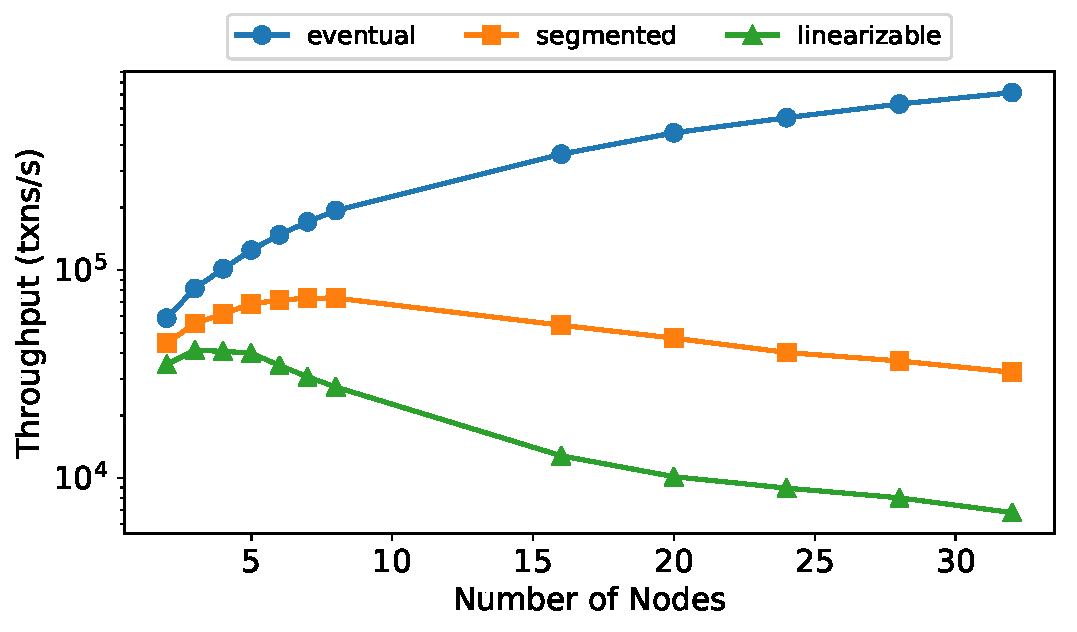
\includegraphics[width=\columnwidth]{figures/vary_nodes.pdf}
  \caption{%
    Throughput of eventually consistent, segmented invariant-confluent, and
    linearizable replication measured against the number of
    nodes.
  }\figlabel{VaryNodes}
\end{figure}

\begin{benchmark}
  In this benchmark, we measure the scale-out of segmented invariant-confluent
  replication. We repeat \benchref{VaryWithdraws} with a 10\% withdrawal rate,
  but this time we vary the number of servers we use to replicate our object.
  When we replicate with $n$ servers, we use $3n$ clients (the $3$ colocated
  clients on each server) as part of the workload. The results are shown in
  \figref{VaryNodes}.

  Eventually consistent replication scales perfectly with the number of nodes,
  confirming the results in~\cite{bailis2014coordination}. With eventually
  consistent replication, servers do not coordinate at all, so they are
  completely unaffected by the number of servers. Linearizable replication, on
  the other hand, scales up to about 3-5 servers before performance begins to
  decrease. These numbers are consistent with typical deployments of
  state-machine replication protocols like Paxos~\cite{chandra2007paxos}.
  Because all messages are sent to the leader, the leader becomes the
  bottleneck as the number of servers and clients increases. Moreover, the
  leader must wait for responses from more servers, increasing the latency of
  the slowest response which in turn decreases throughput.
  Segmented invariant-confluent replication scales up to about 6-8 servers
  before succumbing to the same scalability bottlenecks as linearizable
  replication.

  These results highlight the importance of coordination avoidance in
  distributed databases. While segmented invariant-confluent replication scales
  out slightly better than linearizable replication, both scale significantly
  worse than eventually consistent replication even for a very low (i.e.\ 10\%)
  withdrawal workload. This demonstrates that even a small amount of
  coordination can significantly reduce the scalability of a system.
\end{benchmark}
